\chapter{Einleitung}

\section{Aufgabe/Motivation}
Ziel des Versuchs ist die Untersuchung von freien und erzwungenen Schwingungen eines Drehpendels sowie die Bestimmung der Dämpfungskonstante $\delta$ mittels verschiedener Methoden. Dazu werden zunächst die Periodendauer ungedämpfter Schwingungen gemessen, anschließend die Abnahme der Amplitude bei gedämpften Schwingungen verfolgt und schließlich die Resonanzkurven bei erzwungenen Schwingungen untersucht. Der Vergleich der aus unterschiedlichen Verfahren gewonnenen Werte ermöglicht eine Bewertung der Messmethoden und vertieft das Verständnis für das Verhalten gedämpfter und getriebener Schwingungen.

\section{Physikalische Grundlagen}
\cite{skript25}
Ein Drehpendel ist einem System harmonischer Schwingungen vergleichbar, wobei die Schwingungen in der Praxis stets durch Reibung oder andere Widerstände gedämpft werden. In diesem Versuch erfolgt die Dämpfung durch eine Wirbelstrombremse: Elektromagnete erzeugen ein Magnetfeld, in dem das bewegte Pendel Wirbelströme induziert. Nach der Lenz’schen Regel wirken diese Ströme der Bewegung entgegen und bremsen die Rotation des Pendels.  

Für eine freie, gedämpfte Schwingung des Pendels gilt die zeitliche Entwicklung der Amplitude:
\begin{equation}
a(t) = a_0 \, e^{-\delta t} \, \sin(\omega_f t),
\end{equation}
wobei $\delta$ die Dämpfungskonstante und $\omega_f$ die Kreisfrequenz der gedämpften Schwingung ist. In den Umkehrpunkten vereinfacht sich dies zu
\begin{equation}
a(t) = a_0 \, e^{-\delta t}.
\end{equation}

Die Dämpfungskonstante $\delta$ kann über den exponentiellen Abfall der Amplitude bestimmt werden, beispielsweise über die Halbwertszeit $t_{1/2}$:
\begin{equation}
\delta = \frac{\ln 2}{t_{1/2}}.
\end{equation}

Die Kreisfrequenzen der ungedämpften Schwingung $\omega_0$ und der gedämpften Schwingung $\omega_f$ stehen in folgendem Zusammenhang:
\begin{equation}
\omega_f = \sqrt{\omega_0^2 - \delta^2}.
\end{equation}

Wird das Pendel durch ein periodisches Drehmoment angeregt, stellt sich nach dem Einschwingen eine stationäre Schwingung mit der Frequenz des Erregers ein. Die Amplitude dieser erzwungenen Schwingung hängt von der Erregerfrequenz $\omega$ ab und kann durch die Resonanzkurve beschrieben werden:
\begin{equation}
b(\omega) = \frac{A \, \omega_0^2}{\sqrt{(\omega_0^2 - \omega^2)^2 + (2 \delta \, \omega)^2}}.
\end{equation}

Das Maximum der Amplitude tritt bei der Resonanzfrequenz $\omega'$ auf:
\begin{equation}
\omega' = \sqrt{\omega_0^2 - 2 \delta^2}.
\end{equation}

\begin{figure}[h!]
    \centering
    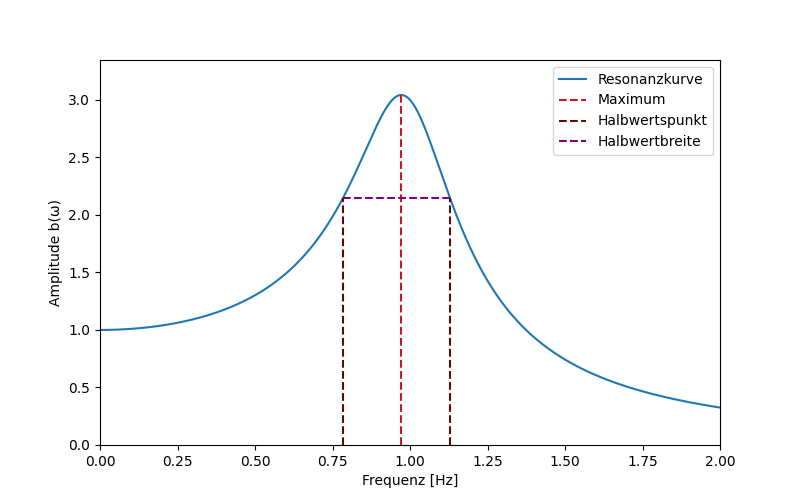
\includegraphics[width=0.5\textwidth]{img/13/Resonanzkurve_allgemein.png}
    \caption{ Schematische Resonanzkurve $b(\omega)$ eines gedämpften, erzwungenen Oszillators.}
    \label{fig:resonanzkurve}
\end{figure}

\textcolor{red}{HIER UNBEDINGT NOCH DIE BENENNUNG DER PUNKTEN IN DER ABBILDUNG MACHEN!}

Wichtige Größen zur Charakterisierung der Resonanzkurve sind die Halbwertsbreite $H$ und die Resonanzüberhöhung:
\begin{equation}
H = \omega_2 - \omega_1 = 2 \delta, \quad \frac{b(\omega')}{b(\omega \to 0)} = \frac{\omega_0}{2 \delta}.
\end{equation}

Durch Messung der freien und erzwungenen Schwingungen lassen sich die Dämpfungskonstante $\delta$ und die Eigenfrequenz des Drehpendels auf mehreren Wegen bestimmen und miteinander vergleichen.
